%%%%%%%%%%%%%%%%%%%%%%%%%%%%%%%%%%%%%%%%%%%%%%%%%%%
%
%  Author: Jacob Vaughn
%  
%  Last Updated: 1/13/2024
%
%%%%%%%%%%%%%%%%%%%%%%%%%%%%%%%%%%%%%%%%%%%%%%%%%%%
%%%%%%%%%%%%%%%%%%%%%%%%%%%%%%%%%%%%%%%%%%%%%%%%%%%%%%%%%%%%%%%%%%%%%%
%%                       EXPERIMENTAL SETUP
%%%%%%%%%%%%%%%%%%%%%%%%%%%%%%%%%%%%%%%%%%%%%%%%%%%%%%%%%%%%%%%%%%%%%

\chapter{EXPERIMENTAL APPROACH \& OBJECTIVES}

\section{Experimental Control and Efficiency Improvements} 

Stuff about ACE2.0 controls

\subsection{Active Mach Number Control}

Stuff

\subsection{Feedback-Controlled Mach Number Selection}

Inputting Mach number into PLC to actively adjust to desired Mach number within some tolerance. Result of above ACE2.0 development.

\subsection{Uncerntainty Quantification}

Unsure how to proceed

\subsection{Reynolds Number Control Scheme}

Control $P_{0}$ to maintain constant Re/m during Mach sweep. Look into anticapatory change in Re/m for potential delayed response time in $P_{0}$, and look into potential proportional Re/m change to model acceleration or altitude change.

Mathematic model predictive controller or preprogrammed controller will be implemented until an adequate PID controller can be developed.

\begin{equation}
    Re/m = \frac{\rho U}{\mu}
\end{equation}
\begin{equation}
    \frac{T_0}{T} = (1+\frac{\gamma-1}{2}M^2) = F
\end{equation}
\begin{equation}
    \frac{P_0}{P} = (1+\frac{\gamma-1}{2}M^2)^{\frac{\gamma}{\gamma+1}} = F^{\frac{\gamma}{\gamma+1}}
\end{equation}
\begin{equation}
    \rho = \frac{P}{R T} = \frac{P_0 F^{\frac{-\gamma}{\gamma-1}}}{R T_0 F^{-1}} = \frac{P_0}{R T_0 F^{\frac{1}{\gamma-1}}}
\end{equation}
\begin{equation}
    U = M \sqrt{\gamma R T} = M F^{-\frac{1}{2}} \sqrt{\gamma R T_0}
\end{equation}
\begin{equation*}
    Re/m = \frac{\rho U}{\mu} = \frac{1}{\mu} \frac{P_0}{R T_0 F^{\frac{1}{\gamma-1}}} M F^{-\frac{1}{2}} \sqrt{\gamma R T_0}
\end{equation*}
\begin{equation}
    Re/m = \sqrt{\frac{\gamma}{R T_0}} \frac{M P_0}{\mu} F^{-\frac{\gamma+1}{2(\gamma -1}}
\end{equation}

For constant Re/m assuming $\gamma, R, T_0 = const.$ and with $\frac{dF}{dt} = (\gamma-1)M \frac{dM}{dt}$:
\begin{equation}
    \frac{d(Re/m)}{dt} = 0 = P_0 \frac{dM}{dt} + M \frac{dP_0}{dt} - \frac{M P_0}{\mu} \frac{d\mu}{dt} - \frac{\gamma+1}{2} M^2 P_0 F^{-1} \frac{dM}{dt}
\end{equation}

Sutherland's Law with $T_\mu = 273$, $S_\mu = 111$, and $\mu_0 = 1.716 \times 10^{-5}$:
\begin{equation}
    \mu = \mu_0 \frac{T_\mu+S_\mu}{T+S_\mu} \left( \frac{T}{T_\mu} \right)
\end{equation}
\begin{equation}
    \mu = \frac{\mu_0(t_\mu+S_\mu)}{T_\mu^{\frac{3}{2}}} \frac{T_0^{\frac{3}{2}} F^{-\frac{3}{2}}}{T_0 F^{-1}+S_\mu}
\end{equation}
\begin{equation}
    \frac{\frac{d\mu}{dt}}{\mu} = (\gamma-1) M F^{-1} \frac{dM}{dt} \left( \frac{T_0 F^{-1}}{T_0 F^{-1} + S_\mu}-\frac{3}{2} \right)
\end{equation}

Substiuting and solving for $\frac{dP_0}{dt}$:
\begin{equation}
    \frac{dP_0}{dt} = P_0 M F^{-1} \frac{dM}{dt} \left[ (\gamma-1) \left( \frac{T_0 F^{-1}}{T_0 F^{-1} + S_\mu} - \frac{3}{2} \right) + \frac{\gamma+1}{2} - \frac{1}{M^2 F^{-1}} \right]
\end{equation}

\section{Nozzle Noise and Uniformity Characterization with Hysteresis}

In order to establish a baseline for future work within the ACE2.0 facility, a pitot survey was performed to measure and characterize the freestream noise and uniformity throuhgout the nozzle. Utilize pitot probe/rake and kulites mounted on traverse to characterize entire nozzle exit plane and centerline into nozzle up to 24??? inches upstream of nozzle exit.

Sweep Re/m and Mach to explore hysteresis of noise and maybe uniformity. Begin with Re/m sweep up and back down in current ACE.

\section{Model Flow Characteristics Hysteresis During Mach Trajectory and Oscillation}

This objective serves as a demonstration of capabilities for ACE2.0. 

Look into hysteresis of boundary layers, shock interactions, and subsequent surface heat flux. 

Use AGARD-B or Fin Cone model for public and HARV for army and verbal?

\begin{figure}[ht]
    \centering
    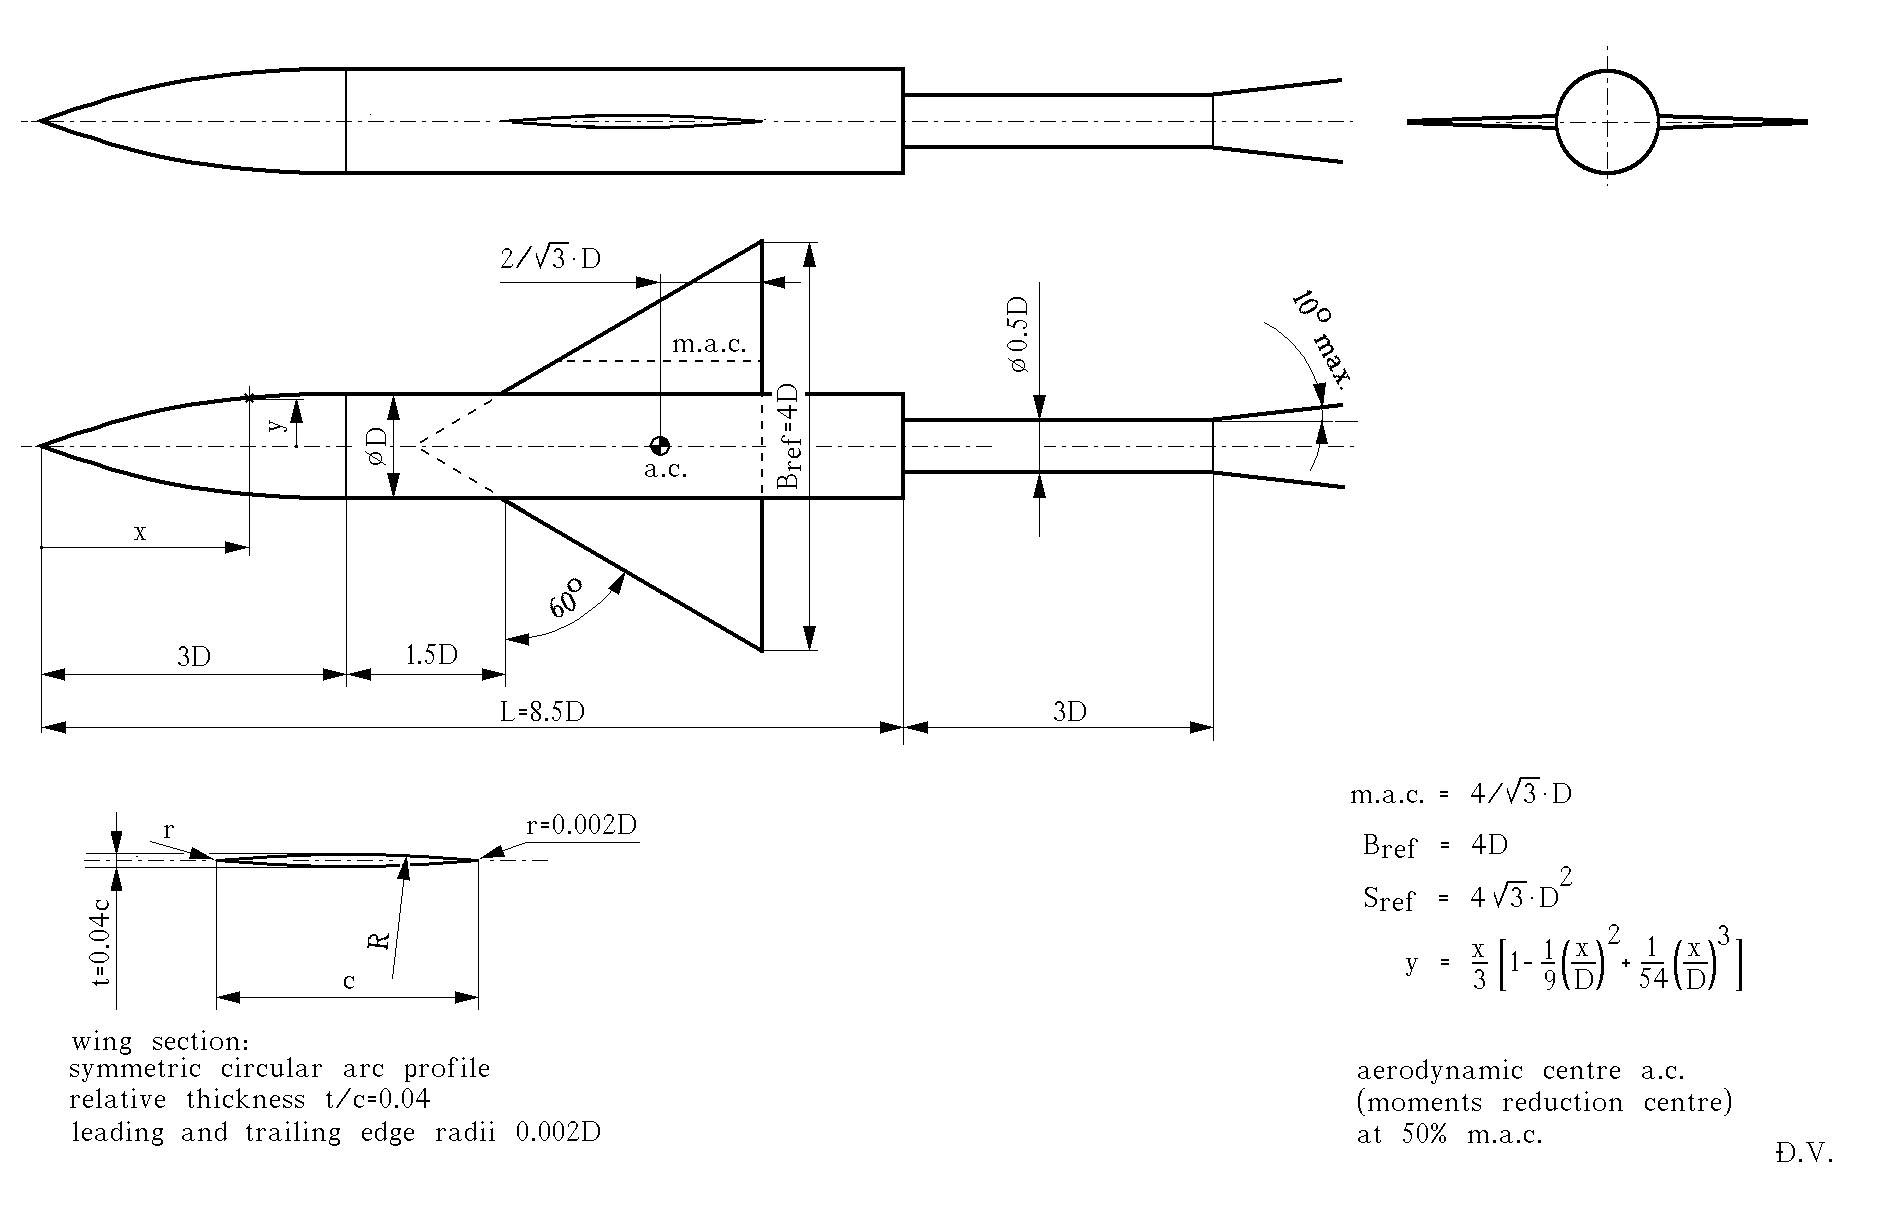
\includegraphics[width=6.5in]{agard_b}
    \caption{AGARD-B check model drawing}
    \label{fig:agard_b}
\end{figure}

